% !TeX TXS-program:compile = txs:///lualatex

\documentclass[a4paper,11pt]{article}
\usepackage[revgoku]{cp-base}
\graphicspath{{./graphics/}}
%variables
\donnees[
	classe={1\up{ère} 2M2},matiere={[SPÉ.MATHS]},mois=Janvier,annee=2022,typedoc=CHAP,numdoc=5
]
%formatage
\author{Pierquet}
\title{\nomfichier}
\hypersetup{pdfauthor={Pierquet},pdftitle={\nomfichier},allbordercolors=white,pdfborder=0 0 0,pdfstartview=FitH}
\lhead{\entete{\matiere}}
\chead{\entete{\lycee}}
\rhead{\entete{\classe{} - \mois{} \annee}}
\lfoot{\pied{\matiere}}
\cfoot{\logolycee{}}
\rfoot{\pied{\numeropagetot}}
%divers

\begin{document}

\pagestyle{fancy}

\part{CH05 - Probabilités conditionnelles, indépendance - Exercices}

\smallskip

\exonum{}

\medskip

En vue de sa prochaine brochure d'information sur les dangers des Réseaux Sociaux, un lycée a fait remplir un questionnaire à chacun des \num{2000}~élèves, répartis dans les sections de seconde, première et terminale. On obtient la répartition : 

\begin{itemize}
	\item un quart des élèves est en terminale ; 
	\item 35\,\% des élèves sont en première ; 
	\item tous les autres sont en seconde ; 
	\item parmi les élèves de terminale, 70\,\% utilisent régulièrement les Réseaux Sociaux ; 
	\item 630 élèves sont des élèves de première qui utilisent régulièrement les Réseaux Sociaux.
	\item \num{1740}~élèves utilisent régulièrement les Réseaux Sociaux.
\end{itemize}

Cette enquête permet de modéliser le choix d'un élève du lycée. On choisit au hasard un questionnaire d'élève en supposant que ce choix se fait en situation d'équiprobabilité. On note :

\begin{itemize}
	\item $S$ l'évènement \og le questionnaire est celui d'un élève en classe de seconde \fg ;
	\item $E$ l'évènement \og le questionnaire est celui d'un élève en classe de première \fg ;
	\item $T$ l'évènement \og le questionnaire est celui d'un élève en classe de terminale \fg ;
	\item $R$ l'évènement \og le questionnaire est celui d'un élève qui utilise régulièrement les Réseaux Sociaux (RS) \fg.
\end{itemize}

\begin{enumerate}
	\item Compléter le tableau d'effectifs ci-dessous.
	
	\smallskip
	
	\begin{tblr}{%
			width=\linewidth,colspec={l*{4}{X[c]}},
			vline{1}={2-Z}{solid},vline{2-Z}={solid},hline{1}={2-Z}{solid},hline{2-Z}={solid},
			rows={font=\sffamily}
		}
		& Seconde & Première & Terminale & Total\\
		Utilise régulièrement les RS 		&	&630&	&		\\
		N'utilise pas régulièrement les RS 	&	&	&	&		\\
		Total 								&	&	&	&2\,000	\\
	\end{tblr}
	\item Déterminer la probabilité d'obtenir le questionnaire d'un élève de seconde qui utilise régulièrement les RS. 
	\item Calculer la probabilité de $R$ sachant $T$, notée $p_{T}(R)$, et interpréter ce résultat à l'aide d'une phrase. 
	\item Calculer la probabilité que le questionnaire choisi soit celui d'un élève qui n'utilise pas les RS. 
	\item Le questionnaire est celui d'un élève qui utilise régulièrement les RS.
	
	Montrer que la probabilité que ce soit le questionnaire d'un élève de première est égale à $\frac{21}{58}$.
\end{enumerate}

\medskip

\exonum{}

\medskip

Une entreprise financière est divisée en deux secteurs ; 65\,\% de son personnel travaille dans le secteur A et 35\,\% dans le secteur B. Cette entreprise s'intéresse au niveau de stress de son personnel.
 
Une enquête, menée sous la forme d'un questionnaire informatisé, est réalisée au sein de l'entreprise. Le questionnaire est proposé de manière anonyme aux salariés des deux secteurs. Cette enquête révèle que pour le secteur A, 20\,\% du personnel se dit stressé, tandis que, dans le secteur B, ce taux est de 30\,\%. 

On choisit au hasard le questionnaire d'un employé de l'entreprise, chacun ayant la même probabilité d'être choisi. On note : 

\begin{itemize}
	\item A : \og le questionnaire est celui d'un employé du secteur A \fg. 
	\item B : \og le questionnaire est celui d'un employé du secteur B \fg. 
	\item S : \og le questionnaire est celui d'un employé stressé \fg.
\end{itemize}
 
\begin{enumerate}
	\item Construire un arbre pondéré décrivant la situation. 
	\item Calculer la probabilité que le questionnaire choisi soit celui d'un employé qui travaille dans le secteur B et qui est stressé. 
	\item L'entreprise examine l'opportunité d'installer une salle de relaxation. Si le taux d'employés stressés est strictement supérieur à 25\,\%, cette salle sera installée.
	 
	L'entreprise implantera-t-elle la salle de relaxation ? Justifier la réponse. 
	\item Sachant que le questionnaire choisi est celui d'un employé stressé, quelle est la probabilité qu'il travaille dans le secteur A ? (le résultat sera arrondi à $10^{-2}$)
\end{enumerate} 

\medskip

\exonum{}

\medskip

Un restaurant propose à sa carte deux types de dessert :

\begin{itemize}
	\item[$\bullet~$] un assortiment de macarons, choisi par 50\,\% des clients; 
	\item[$\bullet~$] une part de tarte tatin, choisie par 30\,\% des clients.
\end{itemize}
 
20\,\% des clients ne prennent pas de dessert et aucun client ne prend plusieurs desserts. Le restaurateur constate :

\begin{itemize}
	\item que parmi les clients ayant pris un assortiment de macarons, 80\,\% prennent un café ; 
	\item que parmi les clients ayant pris une part de tarte tatin, 60\,\% prennent un café; 
	\item que parmi les clients n'ayant pas pris de dessert, 90\,\% prennent un café.
\end{itemize}

On interroge au hasard un client de ce restaurant. On note $p$ la probabilité associée à cette expérience aléatoire. On note :

\begin{itemize}
	\item $M$ l'évènement : \og Le client prend un assortiment de macarons \fg{} ; 
	\item $T$ l'évènement : \og Le client prend une part de tarte tatin \fg{} ; 
	\item $P$ l'évènement : \og Le client ne prend pas de dessert \fg{} ; 
	\item $C$ l'évènement: \og Le client prend un café \fg{} et $\overline{C}$ l'évènement contraire de $C$.
\end{itemize}
 
\begin{enumerate}
	\item En utilisant les données de l'énoncé, préciser la valeur de $p(T)$ et celle de $p_{T}(C)$, probabilité de l'évènement $C$ sachant que $T$ est réalisé. 
	\item Recopier et compléter l'arbre ci-dessous: 
	
	\begin{center}
		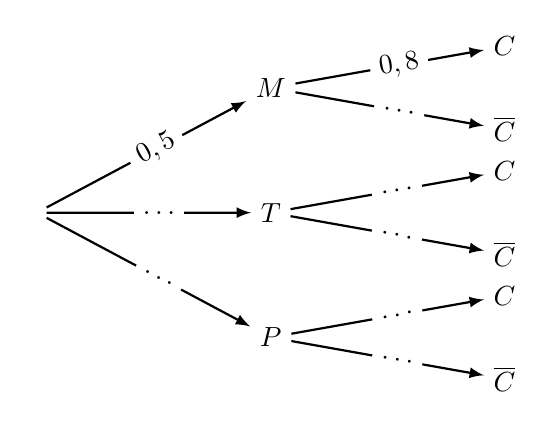
\begin{tikzpicture}[scale=0.66]
		\tikzstyle{fleche}=[->,>=latex,thick]
		\tikzstyle{noeud}=[]
		\tikzstyle{feuille}=[]
		\tikzstyle{etiquette}=[pos=0.55,sloped,fill=white]
		
		\def\DistanceInterNiveaux{3}
		\def\DistanceInterFeuilles{1}
		
		\def\NiveauA{(0)*\DistanceInterNiveaux}
		\def\NiveauB{(1.5)*\DistanceInterNiveaux}
		\def\NiveauC{(3)*\DistanceInterNiveaux}
		\def\InterFeuilles{(-0.8)*\DistanceInterFeuilles}
		
		\node[noeud] (R) at ({\NiveauA},{(4)*\InterFeuilles}) {$ $};
		\node[noeud] (Ra) at ({\NiveauB},{(1)*\InterFeuilles}) {$M$};
		\node[feuille] (Raa) at ({\NiveauC},{(0)*\InterFeuilles}) {$C$};
		%\node[feuille] (Rab) at ({\NiveauC},{(1)*\InterFeuilles}) {$C_{n+1}$};
		\node[feuille] (Rac) at ({\NiveauC},{(2)*\InterFeuilles}) {$\overline{C}$};
		\node[noeud] (Rb) at ({\NiveauB},{(4)*\InterFeuilles}) {$T$};
		\node[feuille] (Rba) at ({\NiveauC},{(3)*\InterFeuilles}) {$C$};
		%\node[feuille] (Rbb) at ({\NiveauC},{(4)*\InterFeuilles}) {$B_{n+1}$};
		\node[feuille] (Rbc) at ({\NiveauC},{(5)*\InterFeuilles}) {$\overline{C}$};
		\node[noeud] (Rc) at ({\NiveauB},{(7)*\InterFeuilles}) {$P$};
		\node[feuille] (Rca) at ({\NiveauC},{(6)*\InterFeuilles}) {$C$};
		%\node[feuille] (Rcb) at ({\NiveauC},{(7)*\InterFeuilles}) {$A_{n+1}$};
		\node[feuille] (Rcc) at ({\NiveauC},{(8)*\InterFeuilles}) {$\overline{C}$};
		
		\draw[fleche] (R)--(Ra) node[etiquette] {$\num{0,5}$};
		\draw[fleche] (Ra)--(Raa) node[etiquette] {$\num{0,8}$};
		\draw[fleche] (Ra)--(Rac) node[etiquette] {$\ldots$};
		\draw[fleche] (R)--(Rb) node[etiquette] {$\ldots$};
		\draw[fleche] (Rb)--(Rba) node[etiquette] {$\ldots$};
		\draw[fleche] (Rb)--(Rbc) node[etiquette] {$\ldots$};
		\draw[fleche] (R)--(Rc) node[etiquette] {$\ldots$};
		\draw[fleche] (Rc)--(Rca) node[etiquette] {$\ldots$};
		\draw[fleche] (Rc)--(Rcc) node[etiquette] {$\ldots$};
		\end{tikzpicture}
	\end{center}
	\item  
		\begin{enumerate}
			\item Exprimer par une phrase ce que représente l'évènement $M \cap C$ puis calculer $p(M \cap C)$.
			\item Montrer que $p(C) = \num{0,76}$.
		\end{enumerate} 
	\item Quelle est la probabilité que le client prenne un assortiment de macarons sachant qu'il prend un café ?
	\item Un assortiment de macarons est vendu 6\,€, une part de tarte tatin est vendue 7\,€, et un café est vendu 2\,€.
	 
	Chaque client prend un seul plat au prix unique de 18\,€, ne prend pas plus d'un dessert ni plus d'un café.
 
	\begin{enumerate}
		\item Quelles sont les six valeurs possibles pour la somme totale dépensée par un client? 
		\item Reproduire et compléter le tableau ci-dessous donnant la loi de probas de la somme totale dépensée :
		
		\smallskip
		
		\begin{tabularx}{\linewidth}{|l|*{6}{>{\centering \arraybackslash}X|}}\hline
			Sommes $s_{i}$& 18 &20 &24 &\ldots&\ldots&\ldots\\ \hline
			$p\left(s_{i}\right)$&0,02&0,18&\ldots&&&\\ \hline 
		\end{tabularx}
	
		\smallskip
	\item Calculer l'espérance mathématique de cette loi et interpréter ce résultat. 
	\end{enumerate}
\end{enumerate}
%
%\medskip
%
%\exonum{}
%
%\medskip
%
%Une salle de jeu comporte deux consoles identiques proposant le même jeu. Un jour l'une des deux est déréglée.
%
%Les joueurs ne peuvent pas savoir laquelle des deux est déréglée. 
%
%\begin{enumerate}
%	\item Ce jour-là, un joueur choisit au hasard l'une des deux consoles et il joue une partie sur cette console.
%	
%	On note :
%	\begin{itemize}[topsep=1pt]
%		\item $D$ l'évènement \og le joueur choisit la console déréglée\fg{} et $\overline{D}$ l'évènement contraire ; 
%		\item $G$ l'évènement \og le joueur gagne la partie \fg{} et $\overline{G}$  l'évènement contraire. 
%	\end{itemize}
%	
%	Cette situation aléatoire est modélisée par l'arbre incomplet suivant, dans lequel figure certaines probas. 
%	
%	\begin{center}
%		\begin{tikzpicture}[xscale=0.9,yscale=0.9]
%			\tikzstyle{fleche}=[->,>=latex,thick]
%			\tikzstyle{noeud}=[]
%			\tikzstyle{feuille}=[]
%			\tikzstyle{etiquette}=[pos=0.55,sloped,fill=white]
%			
%			\def\DistanceInterNiveaux{3}
%			\def\DistanceInterFeuilles{0.85}
%			
%			\def\NiveauA{(0)*\DistanceInterNiveaux}
%			\def\NiveauB{(1.25)*\DistanceInterNiveaux}
%			\def\NiveauC{(2.5)*\DistanceInterNiveaux}
%			\def\InterFeuilles{(-1)*\DistanceInterFeuilles}
%			
%			\node[noeud] (R) at ({\NiveauA},{(1.5)*\InterFeuilles}) {$\Omega$};
%			\node[noeud] (Ra) at ({\NiveauB},{(0.5)*\InterFeuilles}) {$D$};
%			\node[feuille] (Raa) at ({\NiveauC},{(0)*\InterFeuilles}) {$G$};
%			\node[feuille] (Rab) at ({\NiveauC},{(1)*\InterFeuilles}) {$\overline{G}$};
%			\node[noeud] (Rb) at ({\NiveauB},{(2.5)*\InterFeuilles}) {$\overline{D}$};
%			\node[feuille] (Rba) at ({\NiveauC},{(2)*\InterFeuilles}) {$G$};
%			\node[feuille] (Rbb) at ({\NiveauC},{(3)*\InterFeuilles}) {$\overline{G}$};
%			
%			\draw[fleche] (R)--(Ra) node[etiquette] {${0,5}$};
%			\draw[fleche] (Ra)--(Raa) node[etiquette] {${0,7}$};
%			\draw[fleche] (Ra)--(Rab) node[etiquette] {$\ldots$};
%			\draw[fleche] (R)--(Rb) node[etiquette] {$ \ldots$};
%			\draw[fleche] (Rb)--(Rba) node[etiquette] {${0,2}$};
%			\draw[fleche] (Rb)--(Rbb) node[etiquette] {$\ldots$};
%		\end{tikzpicture}
%	\end{center}
%	
%	\begin{enumerate}
%		\item Compléter l'arbre de probabilité. 
%		\item Calculer la probabilité de l'évènement \og  le joueur choisit la console déréglée et il gagne \fg.
%		\item Calculer la probabilité de l'évènement \og le joueur choisit la console non déréglée et il gagne \fg.
%		\item Montrer que la probabilité que le joueur gagne est égale à $0,45$.
%		\item Calculer la probabilité que le joueur ait choisit la console déréglée sachant qu'il a gagné.
%	\end{enumerate}
%	\item Les évènements D et G sont-ils indépendants ? Justifier la réponse.
%	\item Calculer la probabilité de l'événement \og le joueur gagne trois parties de suite \fg{}.
%\end{enumerate}
%
%\medskip
%
%\exonum{}
%
%\medskip
%
%Un nouveau bachelier souhaitant souscrire un prêt automobile pour l'achat de sa première voiture, a le choix entre les trois agences bancaires de sa ville : agence A, agence B et agence C. Après vérification, on a constaté que :
%%
%\begin{itemize}
%	\item 20\:\% des prêts sont souscrits dans l'agence A,
%	\item 45\:\% des prêts sont souscrits dans l'agence B,
%	\item les autres prêts étant souscrits dans l'agence C. 
%\end{itemize}
%%  
%On suppose que tous les clients souscrivent à une assurance dans l'agence où le prêt est souscrit.
%
%Deux types de contrats sont proposés : le contrat tout risque, dit \emph{Zen} et le deuxième contrat appelé \emph{Speed}. 
%
%\medskip
%
%\hspace{5mm}-- 80\,\% des clients de l'agence A ayant souscrit un prêt automobile, souscrivent une assurance \emph{Zen}.
%
%\hspace{5mm}-- 30\,\% des clients de l'agence B ayant souscrit un prêt automobile, souscrivent une assurance \emph{Zen}. 
%
%\hspace{5mm}-- $\nicefrac{2}{7}$ des clients de l'agence C ayant souscrit un prêt automobile, souscrivent une assurance \emph{Speed}.
%
%\smallskip 
%
%On interroge au hasard un client d'une de ces trois banques ayant souscrit un contrat d'assurance automobile. 
%
%On considère les évènements suivants :
%
%\begin{itemize}
%	\item A : \og le prêt a été souscrit dans l'agence A \fg{},
%	\item B : \og le prêt a été souscrit dans l'agence B \fg{},
%	\item C : \og le prêt a été souscrit dans l'agence C \fg{}, 
%	\item Z : \og le contrat d'assurance \emph{Zen} a été souscrit \fg{}, 
%	\item S : \og le contrat d'assurance \emph{Speed} a été souscrit \fg{}.
%\end{itemize}
%
%\begin{enumerate}
%	\item Représenter la situation à l'aide d'un arbre pondéré. 
%	\item Déterminer la probabilité que le client interrogé ait souscrit un prêt automobile avec une assurance \emph{Zen} dans l'agence A. 
%	\item Vérifier que la probabilité de l'évènement Z est égale à $0,545$. 
%	\item Le client a souscrit une assurance \emph{Zen}. Déterminer la probabilité que le prêt soit souscrit dans l'agence C. 
%\end{enumerate}
%
%\medskip
%
%\exonum{}
%
%\medskip
%
%Un concessionnaire automobile vend deux versions de voitures pour une marque donnée: routière ou break. Pour chaque version il existe deux motorisations : essence ou diesel. Le concessionnaire choisit au hasard un client ayant déjà acheté une voiture. On note : 
%
%\begin{itemize}
%	\item $R$ l'évènement: \og la voiture achetée est une routière \fg{} ;
%	\item $B$ l'évènement: \og la voiture achetée est une break \fg{}; 
%	\item $E$ l'évènement : \og la voiture est achetée avec une motorisation essence \fg{} ;
%	\item $D$ l'évènement : \og la voiture est achetée avec une motorisation diesel \fg. 
%\end{itemize}
%%
%On sait que :
%%
%\begin{itemize}[topsep=1pt]
%	\item[$\bullet~$] 65\:\% des clients achètent une voiture routière. 
%	\item[$\bullet~$] Lorsqu'un client achète une voiture break, il choisit dans 85\:\% des cas la motorisation diesel. 
%	\item[$\bullet~$] $27,3$\:\% des clients achètent une voiture routière avec une motorisation diesel.
%\end{itemize}
%
%\begin{enumerate}
%	\item Quelle est la probabilité $p(R)$ de l'événement $R$ ? 
%	\item 
%	\begin{enumerate}
%		\item Construire l'arbre de probabilité (il sera complété ultérieurement). 
%		\item Démontrer que $P_{R}(D) = 0,42$ (probabilité de $D$ sachant $R$). 
%	\end{enumerate}
%	\item Calculer $p(D)$. 
%	\item Lorsque le concessionnaire a choisi au hasard un client, on note $X$ le prix de vente (en milliers d'euros) de la voiture achetée. Compléter le tableau suivant donnant la loi de probabilité de $X$.
%	
%	\renewcommand{\arraystretch}{1.3}
%	\begin{tabularx}{\linewidth}{|l|*{4}{Y|}}
%		\hline
%		Version &\multicolumn{2}{c}{Routière} &\multicolumn{2}{c}{Break} \\ \hline
%		Motorisation &Essence&Diesel &Essence &Diesel \\ \hline
%		$x_{i}$ : prix de vente (en milliers d'€) &15 &18 &17 &20\\ \hline 
%		$P_{i}$ : probabilité&& $0,273$&&\\ \hline
%	\end{tabularx} 
%	
%	Calculer l'espérance mathématique de $X$. Quelle interprétation peut-on en donner ? 
%\end{enumerate}
%
%\medskip
%
%\exonum{}
%
%\medskip
%
%Une boîte de chocolats contient 50\,\% de chocolats au lait, 30\,\% de chocolats noirs et 20\,\% de chocolats blancs. Tous les chocolats de la boîte sont de même forme et d'emballage identique. 
%
%Ils sont garnis soit de praliné soit de caramel et, parmi les chocolats au lait, 56\,\% sont garnis de praliné.
%
%On choisit au hasard un chocolat de la boîte. On suppose que tous les choix sont équiprobables. On note :
%%
%\begin{itemize}
%	\item[$\bullet~$] L : l'évènement \og le chocolat choisi est au lait \fg{} ; 
%	\item[$\bullet~$] N : l'évènement \og le chocolat choisi est noir \fg{} ; 
%	\item[$\bullet~$] B : l'évènement \og le chocolat choisi est blanc \fg{} ; 
%	\item[$\bullet~$] P : l'évènement \og le chocolat choisi est garni de praliné \fg{} ; 
%	\item[$\bullet~$] C : l'évènement \og le chocolat choisi est garni de caramel \fg. 
%\end{itemize}
%
%
%\begin{enumerate}
%	\item Traduire les données du problème à l'aide d'un arbre de probabilité. 
%	\item  Donner la probabilité que le chocolat choisi soit garni de praliné sachant que c'est un chocolat au lait. 
%	\item Déterminer la probabilité  que le chocolat choisi soit au lait et garni de praliné. 
%	\item Dans la boîte, 21\,\% des chocolats sont noirs et garnis de praliné. 
%	
%	Montrer que la probabilité que le chocolat choisi soit garni de praliné, sachant que c'est un chocolat noir, est égale à $0,7$. 
%	\item Dans la boîte, 60\,\% des chocolats sont garnis de praliné. 
%	\begin{enumerate}
%		\item Déterminer la probabilité que le chocolat choisi soit blanc et garni de praliné. 
%		
%		\item En déduire la probabilité que le chocolat choisi soit garni de praliné sachant que c'est un chocolat blanc. 
%	\end{enumerate}
%	\item On dispose de deux boîtes de chocolats identiques à celle décrite précédemment. Une personne prend au hasard un chocolat dans la première boîte, puis un chocolat dans la deuxième boîte (les tirages sont indépendants). 
%	
%	Déterminer la probabilité de l'évènement : \og l'un des chocolats choisi est garni de praliné et l'autre est garni de caramel \fg.
%\end{enumerate}
%
%\medskip
%
%\exonum{}
%
%\medskip
%
%Un site Internet offre la possibilité à des particuliers de vendre des objets aux enchères. Pour chaque objet, la durée des enchères dure une semaine. Si une annonce reçoit une enchère, alors la vente de l'objet est obligatoire à la fin des enchères et ce, même si le vendeur juge le prix de vente trop peu élevé.
%
%Sur ce site une étude statistique a montré que :
%
%\begin{itemize}
%	\item[$\bullet$] $\nicefrac{3}{5}$ des annonces reçoivent une première enchère le lendemain de leur parution ; dans  ce cas, 75\,\% des vendeurs sont satisfaits du prix de vente final ;
%	\item[$\bullet$] $\nicefrac{1}{3}$ des annonces reçoit une première enchère au bout de trois jours et, dans ce cas, 57\,\% des vendeurs sont satisfaits du prix de vente final de leur objet ;
%	\item[$\bullet$] les autres annonces ne reçoivent aucune enchère et le vendeur retire alors son objet de la vente. 
%\end{itemize}
%%
%On choisit au hasard une annonce mise en ligne sur le site. On note :
%%
%\begin{itemize}
%	\item[$\bullet$] L : l'évènement \og l'annonce reçoit une première enchère le lendemain de sa parution \fg ; 
%	\item[$\bullet$] T : l'évènement \og  l'annonce reçoit une première enchère au bout de trois jours \fg ; 
%	\item[$\bullet$] A: l'évènement \og l'annonce ne reçoit aucune enchère \fg ; 
%	\item[$\bullet$] S : l'évènement \og le vendeur est satisfait du prix de vente final de son objet \fg ~et $\overline{S}$ son évènement contraire. 
%\end{itemize}
%
%\begin{enumerate}
%	\item Traduire la situation par un arbre de probabilités. 
%	\item Calculer la probabilité que l'annonce ait reçu une première enchère le lendemain de sa parution et que le vendeur soit satisfait du prix de vente final. 
%	\item Démontrer que la probabilité que le vendeur soit satisfait du prix de vente de son objet est $0,64$. 
%	\item Un objet est vendu à un prix qui satisfait son vendeur. Quelle est la probabilité que cet objet ait reçu une première enchère dès le lendemain de la parution de l'annonce (le résultat sera donné sous forme décimale, arrondi au centième) ? 
%	\item Marc a mis en vente le même jour trois jeux vidéo identiques sur ce site. On suppose que les déroulements des enchères sont indépendants les uns des autres.
%	
%	Calculer la probabilité qu'à la fin des enchères, Marc soit satisfait du prix de vente de tous ses jeux vidéo (arrondie au centième). 
%\end{enumerate}
%
%\medskip
%
%\begin{center}
%	\includegraphics[scale=0.20]{chap05_exov2_humour} 
%	
%	{\scriptsize \textit{Le Devin}, Uderzo \& Goscinny}
%\end{center}

\end{document}